\chapter{Multiple and Polynomial Regression}
\label{chap:multiple_poly_regression}

% ========================================
% SECTION 1: INTRODUCTION
% ========================================
\section{Introduction: Beyond a Single Feature}
In Chapter 1, we predicted Package using only CGPA. But in the real world, many factors influence salary: Projects, Internships, Communication Skills, etc.

\begin{definition}
\textbf{Multiple Linear Regression}: A regression model that predicts a target variable using \textbf{two or more} input features.
\end{definition}

\section{Geometric Intuition}
How does the ``Best Fit Line'' change when we add more features?
\begin{itemize}
    \item \textbf{1 Feature}: The model is a \textbf{Line} in 2D space.
    \item \textbf{2 Features}: The model is a \textbf{Plane} in 3D space.
    \item \textbf{3+ Features}: The model is a \textbf{Hyperplane} in N-dimensional space.
\end{itemize}

\begin{figure}[htbp]
\centering
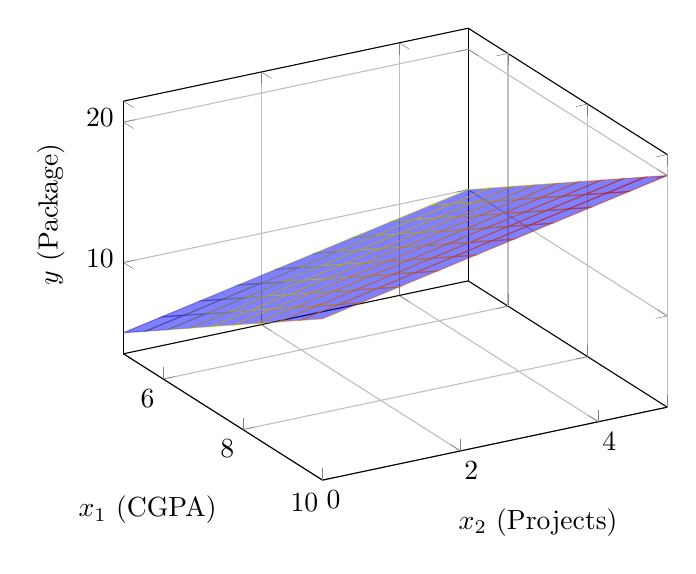
\begin{tikzpicture}
    \begin{axis}[
        view={60}{30},
        xlabel=$x_1$ (CGPA), ylabel=$x_2$ (Projects), zlabel=$y$ (Package),
        width=0.7\textwidth,
        grid=major
    ]
    % Plane: y = 2*x1 + 1*x2 - 5
    \addplot3[surf, opacity=0.5, color=blue, domain=5:10, domain y=0:5, samples=10] {2*x + 1*y - 5};
    \end{axis}
\end{tikzpicture}
\caption{In Multiple Linear Regression with 2 features, the model is a flat plane.}
\label{fig:mlr_plane}
\end{figure}

\begin{figure}[htbp]
\centering
\includegraphics[width=0.8\textwidth]{../02-supervised/assets/multiple_lr_plane.png}
\caption{Another view of the Multiple Linear Regression Plane.}
\label{fig:mlr_plane_img}
\end{figure}

\section{Mathematical Formulation}
The equation extends naturally:
\begin{equation}
    y = \beta_0 + \beta_1 x_1 + \beta_2 x_2 + \ldots + \beta_p x_p
\end{equation}
\begin{itemize}
    \item $\beta_0$: Intercept (baseline value when all features are zero).
    \item $\beta_1, \beta_2, \ldots, \beta_p$: Coefficients (weights for each feature).
    \item For $p$ features, we have $p+1$ parameters to estimate.
\end{itemize}

\section{Matrix Formulation}
For computational efficiency, we express everything using matrices.

\subsection{Setting Up the Matrices}
\begin{itemize}
    \item $\mathbf{Y}$: Vector of target values (size: $n \times 1$).
    $$\mathbf{Y} = \begin{bmatrix} y_1 \\ y_2 \\ \vdots \\ y_n \end{bmatrix}$$
    
    \item $\mathbf{X}$: Design Matrix (size: $n \times (p+1)$). We prepend a column of 1s to handle the intercept $\beta_0$.
    $$\mathbf{X} = \begin{bmatrix} 
    1 & x_{11} & x_{12} & \cdots & x_{1p} \\
    1 & x_{21} & x_{22} & \cdots & x_{2p} \\
    \vdots & \vdots & \vdots & \ddots & \vdots \\
    1 & x_{n1} & x_{n2} & \cdots & x_{np}
    \end{bmatrix}$$
    
    \item $\boldsymbol{\beta}$: Vector of coefficients (size: $(p+1) \times 1$).
    $$\boldsymbol{\beta} = \begin{bmatrix} \beta_0 \\ \beta_1 \\ \vdots \\ \beta_p \end{bmatrix}$$
\end{itemize}

The predicted values are: $\hat{\mathbf{Y}} = \mathbf{X} \boldsymbol{\beta}$

\section{Deriving the Normal Equation (OLS)}
We want to find the $\boldsymbol{\beta}$ that minimizes the Sum of Squared Errors (SSE).

\subsection{Step 1: Define the Error}
The error (residual) vector is:
$$\mathbf{e} = \mathbf{Y} - \hat{\mathbf{Y}} = \mathbf{Y} - \mathbf{X}\boldsymbol{\beta}$$

\subsection{Step 2: Define the Loss Function (SSE)}
The Sum of Squared Errors in matrix form is:
$$E = \mathbf{e}^T \mathbf{e} = (\mathbf{Y} - \mathbf{X}\boldsymbol{\beta})^T (\mathbf{Y} - \mathbf{X}\boldsymbol{\beta})$$

\subsection{Step 3: Expand the Expression}
Using the transpose rule $(AB)^T = B^T A^T$:
$$E = (\mathbf{Y}^T - \boldsymbol{\beta}^T \mathbf{X}^T)(\mathbf{Y} - \mathbf{X}\boldsymbol{\beta})$$

Multiply out (FOIL method):
\begin{align}
E &= \mathbf{Y}^T \mathbf{Y} - \mathbf{Y}^T \mathbf{X}\boldsymbol{\beta} - \boldsymbol{\beta}^T \mathbf{X}^T \mathbf{Y} + \boldsymbol{\beta}^T \mathbf{X}^T \mathbf{X} \boldsymbol{\beta}
\end{align}

\textbf{Key Observation}: The terms $\mathbf{Y}^T \mathbf{X}\boldsymbol{\beta}$ and $\boldsymbol{\beta}^T \mathbf{X}^T \mathbf{Y}$ are both scalars. Thus:
\begin{equation}
E = \mathbf{Y}^T \mathbf{Y} - 2\boldsymbol{\beta}^T \mathbf{X}^T \mathbf{Y} + \boldsymbol{\beta}^T \mathbf{X}^T \mathbf{X} \boldsymbol{\beta}
\label{eq:sse_expanded}
\end{equation}

\subsection{Step 4: Differentiate and Solve}
Taking the derivative w.r.t $\boldsymbol{\beta}$ and setting to zero:
$$-2\mathbf{X}^T \mathbf{Y} + 2\mathbf{X}^T \mathbf{X} \boldsymbol{\beta} = 0$$
$$\mathbf{X}^T \mathbf{X} \boldsymbol{\beta} = \mathbf{X}^T \mathbf{Y}$$
\begin{equation}
\boxed{\boldsymbol{\beta} = (\mathbf{X}^T \mathbf{X})^{-1} \mathbf{X}^T \mathbf{Y}}
\end{equation}

\section{Polynomial Regression}
What if the relationship is curved? We generate new features ($x^2, x^3$).

\textbf{Model with Interaction Terms}:
For 2 features with Degree 2, we get:
$$ y = \beta_0 + \beta_1 x_1 + \beta_2 x_1^2 + \beta_3 x_2 + \beta_4 x_2^2 + \beta_5 (x_1 x_2) $$

\begin{figure}[htbp]
\centering
\includegraphics[width=0.8\textwidth]{../02-supervised/assets/polynomial_degrees_comparison.png}
\caption{Degree 1 (Underfit) vs Degree 2 (Good Fit) vs Degree 20 (Overfit).}
\label{fig:poly_degrees}
\end{figure}

\section{Implementation in Python (Scikit-Learn)}
\begin{lstlisting}[language=Python, caption=Polynomial Regression Pipeline]
from sklearn.preprocessing import PolynomialFeatures
from sklearn.linear_model import LinearRegression
from sklearn.pipeline import Pipeline
import numpy as np

# 1. Create Non-linear Data
X = np.array([1, 2, 3, 4, 5]).reshape(-1, 1)
y = np.array([1, 4, 9, 16, 25]) # y = x^2

# 2. Use Pipeline
pipe = Pipeline([
    ('poly', PolynomialFeatures(degree=2)),
    ('model', LinearRegression())
])
pipe.fit(X, y)
\end{lstlisting}

\section{Implementation from Scratch (Matrix Method)}
\begin{lstlisting}[language=Python, caption=Multiple Linear Regression from Scratch]
import numpy as np

class MeraMultipleLR:
    def __init__(self):
        self.coef_ = None
        self.intercept_ = None
        
    def fit(self, X_train, y_train):
        # 1. Add column of 1s for intercept (Beta_0)
        # X_train shape: (n, m) -> (n, m+1)
        X_b = np.insert(X_train, 0, 1, axis=1)
        
        # 2. Apply Normal Equation: beta = (X^T X)^-1 X^T Y
        # np.linalg.inv computes the inverse
        try:
            betas = np.linalg.inv(np.dot(X_b.T, X_b)).dot(np.dot(X_b.T, y_train))
            
            self.intercept_ = betas[0]
            self.coef_ = betas[1:]
            print(f"Intercept: {self.intercept_}")
            print(f"Coefficients: {self.coef_}")
            
        except np.linalg.LinAlgError:
            print("Error: Matrix is Singular (Not Invertible). Check for multicollinearity.")

    def predict(self, X_test):
        # y_pred = beta_0 + beta_1*x_1 + ...
        # Formula: y = X_test * coef + intercept
        return np.dot(X_test, self.coef_) + self.intercept_
\end{lstlisting}

\section{HOTS: Interview Questions}
\textbf{Q1: What happens if the matrix $(X^T X)$ is not invertible (Singular)?}
\begin{itemize}
    \item The Normal Equation fails. This happens if:
    \begin{enumerate}
        \item \textbf{Multicollinearity}: Features are perfectly correlated (e.g., $x_2 = 2x_1$).
        \item \textbf{More features than samples} ($p > n$).
    \end{enumerate}
    \item \textbf{Fix}: Use Regularization (Ridge) or drop correlated features.
\end{itemize}

\textbf{Q2: How does geometric interpretation change from 2D to 3D?}
\begin{itemize}
    \item \textbf{2D} (1 feature): Line.
    \item \textbf{3D} (2 features): Plane.
    \item \textbf{ND} (3+ features): Hyperplane.
\end{itemize}

\textbf{Q3: Why is Gradient Descent preferred over OLS for Deep Learning?}
\begin{itemize}
    \item Computing $(X^T X)^{-1}$ is $O(n^3)$. For millions of parameters (Deep Learning), this is impossible.
    \item Gradient Descent scales linearly ($O(n)$) and is iterative, making it feasible for massive datasets.
\end{itemize}

\textbf{Q4: Is Polynomial Regression a linear or non-linear model?}
\begin{itemize}
    \item It is a \textbf{Linear Model} because it is linear with respect to the \textit{parameters} ($\beta$). The non-linearity is in the features.
\end{itemize}

\textbf{Q5: Why is feature scaling important in Polynomial Regression?}
\begin{itemize}
    \item Powers like $x^2, x^3$ explode magnitude. $1000^3$ is huge. Numeric instability occurs without scaling.
\end{itemize}
